\documentclass[a4paper]{article}
\usepackage[margin=1in]{geometry} % 设置边距,符合Word设定
\usepackage{ctex}
\usepackage{graphicx}
\usepackage{amsmath}

\usepackage{amssymb}
\usepackage{color}
\usepackage{appendix}
\usepackage{hyperref} %生成引用链接,注:该宏包可能与其他宏包冲突,故放在所有引用的宏包之后
\usepackage{cleveref} %实现图片和表格、公式的引用,cleveref包必须放在hyperref包之后

%%链接设置
\hypersetup{colorlinks = true, %将链接文字带颜色
	    linkcolor = blue, %图表引用颜色设置为蓝色
	    urlcolor = blue,%网页链接为蓝色
            citecolor = blue} %文献引用颜色设置为蓝色

%%参考文献
%\bibliographystyle{plain} %参考文献引用格式
%\newcommand{\upcite}[1]{\textsuperscript{\cite{#1}}} %引用参考文献时,\upcite{1},能标在右上角

%%全文字体
\begin{document}

\subsection{规范理论}

量子力学中的模型由两部分构成,第一部分是系统演化的哈密顿量 $H$, 
第二部分是系统存在的希尔伯特空间 $\mathcal{H}$,往往只需要取态能够存在的空间作为 
$\mathcal{H}$
就足够分析使用,比如粒子生活在周期性的势场中$H = P^2/2m +V\cos(2\pi x/a)$,
由于势场是有周期平移对称性的,猜测应当也具有周期平移的态才合法,定义变换
$T_a \psi(x)=\psi(a+x)$,
于是取$\mathcal{H}_a=\{\psi|\psi\in L^2[-\infty,+\infty], T_a \psi = \psi \}$,
这个空间就够了。



但是在有的情况下,
在全局的$\mathcal{H}$下定义是有用的,比如该粒子与另一非周期的粒子存在相互作用,
于是需要扩展到所有平方可积函数作为$\mathcal{H}$的成员,
这种情况下去研究问题,就需要引入规范结构,
从而将这个周期的粒子“规范”定义于大的希尔伯特空间中,具体的:

定义变换
$T_a \psi(x)=\psi(a+x)$为规范变换,容易得见$H T_a = T_a H$,哈密顿量与规范变换算符相互对易。

合法的态满足:

$$
\left|x+a\right> = \left|x\right>
$$

在大希尔伯特空间 $\mathcal{H}$ 中,并非每个态都是满足以上条件,故为了表示在 $\mathcal{H}_a$ 
以外的态,需要多添加一个数用于标记,比如
取定了一套$\left|x\right>$坐标基矢,则在大希尔伯特空间 $\mathcal{H}$ 中
任意态写作:$\psi(x) = \left<\psi|x\right>$,
取 $n$ 为任意整数,在 $n$ 次 $T_a$ 作用于态$\psi$
后,任意态写作:$\psi'(x) = \left<\psi T_a^n|x\right> \ne \left<\psi|x\right>$,也就是在
大空间上的作用并非平凡的,而作用于$\mathcal{H}_a$上的态
$\psi'(x) = \left<\psi T_a^n|x\right> = \left<\psi|x\right>$
,于是可以用$n=0$ 代表并未对态做过规范变换,$n$表示对态做规范变换的次数,
这样就可以在大的空间中用$\psi_a \in \mathcal{H}_a$ 和一个多余的数 $n$ 来标记某个态,
这样的处理方式让描述系统的空间扩大且多了一个自由度,这样的结构称为规范结构
,同时将周期平移对称性隐含在了规范结构中,有时也称这个系统拥有了规范对称性,
当然多个对称性的系统也可以这样的处理,同时用 $\{n_1,n_2,..n_k\}$ 矢量(gauge sector)来标记系统,
在这个例子中,规范矢量满足整数群Z的对称性,故称这个系统满足整数群Z的规范对称性。

$n$ 在只讨论 $\mathcal{H}_a$ 内的态时时不会产生任何的意义,只有当出现了规范破坏的项,
也就是不满足对应的对称性的项出现时,矢量才有意义。同时,各个物理量也必须满足规范变换下不变,
系统才能是规范不变的。

\subsection{纯 $Z_2$ 格点规范理论}

\begin{figure}[htbp]
    \centering
    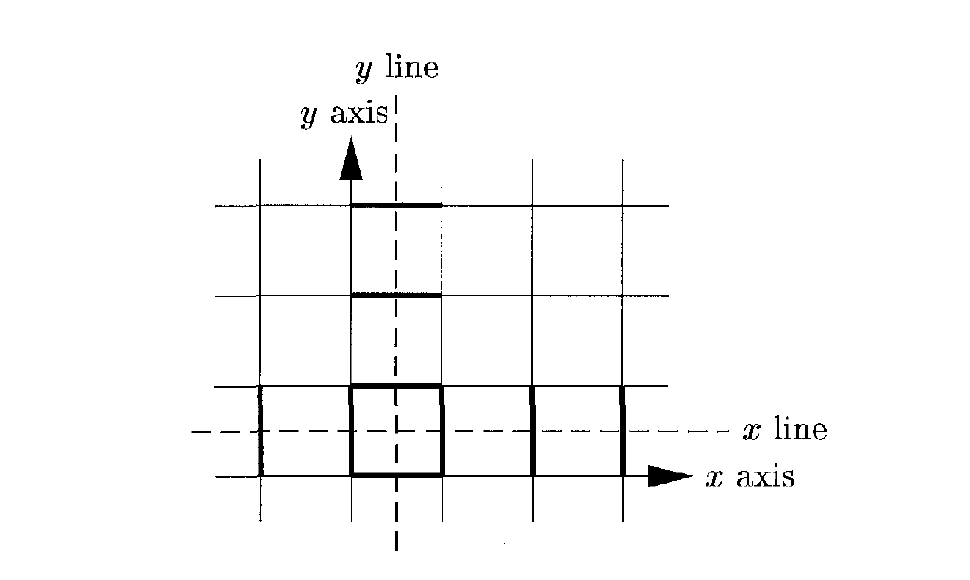
\includegraphics[scale=0.45]{6.png}
    \caption{二维格子以及$Z_2$的定义}
\end{figure}

单纯的$Z_2$系统定义在二维周期边界条件阵列上,在每个棱上有一个场$s_{ij}$(比特),
$i,j$为与其相连的格点,其满足传统二能级结构,也就是说:
系统的大希尔伯特空间可以有$\left|++--...\right>$的形式表达出来, 其中每个比特位对应某条具体的棱,
但是当我们引入某种规范结构,即限制整个二维网的构型到某个子空间中(即小希尔伯特空间),可以在这种
限制下得到某些奇特
的性质,同时也可以探究出哈密顿量的具体形式以及在背后的对称性。

这里用格点定义规范变换$G_i$,定义为对与$i$格点相连的场进行翻转 $s_{ij} -> -s_{ij}$,并且认为$G_i$作用
后的系统与原系统完全一致,没有任何区别,在这样的规范变换定义下,假定
初始状态下$W_i = 1,\forall i\in lattice$,
则对于格点的函数 $G_i = \pm 1$,都对应于一个规范变换,$W_i \rightarrow W_iG_i$,于是$W_i$成为了
这个规范变换的gauge sector,与格点一一对应,同时每个格点的矢量$W_I$满足$Z_2$对称性,称为 $Z_2$ 规范场。

\hspace*{\fill}

\textbf{命题1} 规范变换下,量$F(C)=\prod_{\{i,j\} \in C}s_{i,j}$ 是规范不变量。

\hspace*{\fill}

C是环面上的任意闭合曲线,而任意规范变换一定会是同时操作闭合图形两个棱的翻转,所以这个量在规范变换下
保持不变。

再有,通过这个量可以分别不同的规范变换态,取最小的方格为一个C,则每个方格都可以提供一个用于标记
态的规范自由度的变量,两个构型如果任意一个 $F(square)$ 不相同,就证明这两个构型是不可能通过规范变换
得到,也就是在子空间中这两个态不相同。

\hspace*{\fill}

\textbf{命题2} 规范变换下,量 $\sigma^z_{i,j}$ 是规范不变量。

\hspace*{\fill}

对某个棱的翻转算符$\sigma^z_{i,j}$ 与$W_k$相互对易,所以命题成立。

\hspace*{\fill}

z综上所述,$Z_2$的哈密顿量必须是规范变换下不变的,最简单的写法可以写作:

$$
H = -g \sum_i^{\text{square}} \prod_{(l,m) \in i}  \sigma_{x,(l,m)} -t \sum_{(k,g)} \sigma_{z,(k,g)}  
$$

最后讨论一下子空间中的拓扑简并态,
假设系统有 $Nx \times Ny =N$ 个格点且满足$g \gg t$,并且满足周期对称条件,那么实际上就有2N根棱,不考虑
规范结构,实际可能有$2^{2N}$个态,gauge sector有 $N$ 个变量,共有$2^N$个组合,但是
注意到gauge sector 取 $(1,1,1,1,...)$ 和 $(-1,-1,-1,...)$ 时完全一致,所以有
$2^N/2$个有效组合,故子空间里的态应该有$2\times 2^N$个,通过$F(square)$来标记态的话,拥有 $N$
个变量,但是所有的$\prod_i^{\text{square}} F_i = 1$,也就是说 $F_i$ 只能提供 $2^N/2$ 个标记,
最终认为有 $2^{N+1}/2^{N-1}$ 四个态是完全兼并的,他们的 $F_i$ 完全相同,$H$ 的期望值也完全相同
,在任意局域的$\sigma^z_i$的翻转作用下也没有办法解简并。转换方法需要环绕整个系统的线的沿x翻转或者沿y翻转。
这是一个全局的拓扑操作,给甜甜圈切了一刀,改变了系统的拓扑性质,故也称拓扑简并态。

在$g\gg t\rightarrow 0 $ 时,激发是通过翻转某处$F_i$实现,
称激发子为$Z_2$涡旋,因为$\prod_i^{\text{square}} F_i = 1$涡旋必须成对出现且具有全局的纠缠效应,
这个相称为$Z2$场的解禁闭相(Deconfined Phases),而当$t\gg g\rightarrow 0$ 时$Z2$场退化为Ising模型
激发局域化,称这个相为禁闭相(Confined Phases)。



\subsection{$Z_2$ 格点规范理论与物质的相互耦合}


考虑格点哈密顿量:

$$
H=\sum_i \mu_i \hat{a}_i^{\dagger} \hat{a}_i
$$

观察到格点上的升降算符有对称性 $\hat a_i \rightarrow -\hat a_i$,并不改变其哈密顿量,
猜测定义局域规范变换为 $\hat{\mathcal{V}_i}\equiv e^{i\pi\hat{n}}: \left|n\right>\rightarrow (-1)^n\left|n\right>$,
容易验证$\hat{\mathcal{V}_i} a_i = -a_i \hat{\mathcal{V}_i}$。

玻色子(为了简洁,省略位点角标):

$$
\begin{aligned}
    \hat{\mathcal{V}} a \hat{\mathcal{V}}^\dagger &= e^{-i\pi a^\dagger a}ae^{i\pi a^\dagger a}
    \\& = a - (i\pi)[a^\dagger a,a] +(i\pi)^2[a^\dagger a,[a^\dagger a,a]]/2! +\dots
    \\&= a -(i\pi)(-1)a + (i\pi)^2(-1)^2a/2! + \dots
    \\&= a (1+i\pi+(i\pi)^2/2!+\dots)
    \\&= -a
\end{aligned}
$$

费米子则更为简洁,根据定义$\hat{\mathcal{V}_i} = \sigma^z$,容易验证$\{\sigma^z,\sigma^\pm\} = 0$。
,进一步可以得到$\hat{\mathcal{V}_i}H = H \hat{\mathcal{V}_i}$规范不变,规范变换有意义。
根据前文规范理论,认为规范变换后的态与原态完全一致(实际也满足谐振子模型的基矢相位的任意性),
则得到了这个系统中的gauge sector,每个位点上有一个满足 $Z_2$ 代数结构的规范对称性,
则可以用$(0,0,0,0,..)$等$N$个数表示未加变换的某个选定的能量本征态上($N$ 为格点数),
减少了需要讨论的态的个数。


往往格点之间不相互独立,需要讨论格点间的相互作用时,猜测哈密顿量直接写作:

$$
H=J \sum_{\langle i, j\rangle}\left(\hat{a}_i^{+} 
\hat{a}_j+\text { h.c.}\right)+\sum_i \mu_i \hat{a}_i^{\dagger} \hat{a}_i
$$

沿用上文中关于local规范变换的定义,则有:

$$
\hat{a}_i \rightarrow \hat{\mathcal{V}_i} \hat{a}_i, \quad \hat{a}_i^{+} \rightarrow \hat{a}_i^{+} \hat{\mathcal{V}_i}^{+}
$$

则变换后的哈密顿量写作:

$$
H=J \sum_{\langle i, j\rangle}\left(\hat{a}_i^{\dagger} \hat{\mathcal{V}_i}^{\dagger}\hat{\mathcal{V}_j}\hat{a}_j+\text { h.c. }\right)+\sum_i \mu_i \hat{a}_i^{\dagger} \hat{a}_i
$$

显然直接耦合的哈密顿量相互作用项并不是规范不变的,
前文的规范变换与此哈密顿量不兼容,需要重新考虑哈密顿量的构造以及规范变换的选取。

考虑在两个格点之间引入额外自由度(某个场) $\hat{\mathcal{U}}_{\langle i, j\rangle}$,
并且定义其规范变换的规则$\hat{\mathcal{V}'}_i$,$\hat{\mathcal{V}'}_i$的变换规则
需要与物质场的变换规则$\hat{\mathcal{V}}_i$相关联,最终让$H$在联合的变换下保持不变。

发现,以格点为记号,并且操作只有正负两种选择,操作后认为态并没有发生变化,$Z2$纯规范场刚好
符合要求,定义联合操作:

$$
\begin{aligned}
    W_i &=  \hat{\mathcal{V}}_i \times G_i
    \\&= (-1)^{n_i} \prod_{j}^{[i,j]\text{connect}} \sigma_{z,ij}
\end{aligned}
$$

第一个操作是前文对物质的相位翻转。而第二个操作代表纯$Z_2$规范理论中以某格点为中心对场的翻转。

哈密顿量写作:

$$
\begin{aligned}
    H=&J \sum_{[i,j]\text{connect}}\left(\hat{a}_i^{+} \hat{\sigma}^z_{i, j}\hat{a}_j+\text { h.c. }\right)+\sum_i \mu_i \hat{a}_i^{\dagger} \hat{a}_i
    \\ &-g \sum_i^{\text{square}} \prod_{(l,m) \in i}  \sigma_{x,(l,m)} -t \sum_{(k,g)} \sigma_{z,(k,g)}    
\end{aligned}
$$

容易验证$[W_i,H] = 0$,规范变换成立,值得一提的是,物质场能级之间的相位实际上是$U(1)$的,
所以$Z_2$模型是$U(1)$的一个简单类型,如果物质场写成旋量,实际上还能引入$SU(N)$等更为广泛的规范场,
这种类型的格点规范场论最基础的也最具有意义。$Z2$ 规范场作为一种真实物理的简单情况,同时由于自身非禁闭相
的全局纠缠性质在强关联系统以及拓扑纠错等领域具有重要意义。


\end{document}